\section{Laser peaks detection}
\label{sec:laser-peaks}

Starting from the point $ p_w = \left( x_w, y_w, z_w \right)$ in the 3D space, we reached its projection $p_c = \left( x_c, y_c \right)$ in the sensor reference system. At this point, the error committed while locating the peak, now depends by the technique used. \\

If we consider the general case, without using any sub-pixel approximation, the peak will be consider in the center of the pixel, i.e. located in $p_c$. Accordingly with \cite{th:quattrini}, we can model the distribution of all the possible positions of the peak along a specific direction as a \textit{uniform distribution}, centered in $p_c$, thus we can evaluate the location error with the standard deviation of the distribution, that is
  \begin{equation*}
    \sigma_{p_c} = \sqrt{\frac{\left(b - a\right)^2}{12}}
  \end{equation*}
with $a$ and $b$ the extremes of the range. \\
Let's consider the laser in its coordinates reference system. The use of a line lens allows us to spread the spot energy along a line. From a physical point of view, the signal we obtained in this way, is continuous along the direction of the abscissa, while from a mathematical point of view, the laser can be modelled as a solid Gaussian, like the one shown in Figure \ref{fig:mod-laser-line}.
  \begin{figure}[t!]
    \centering
    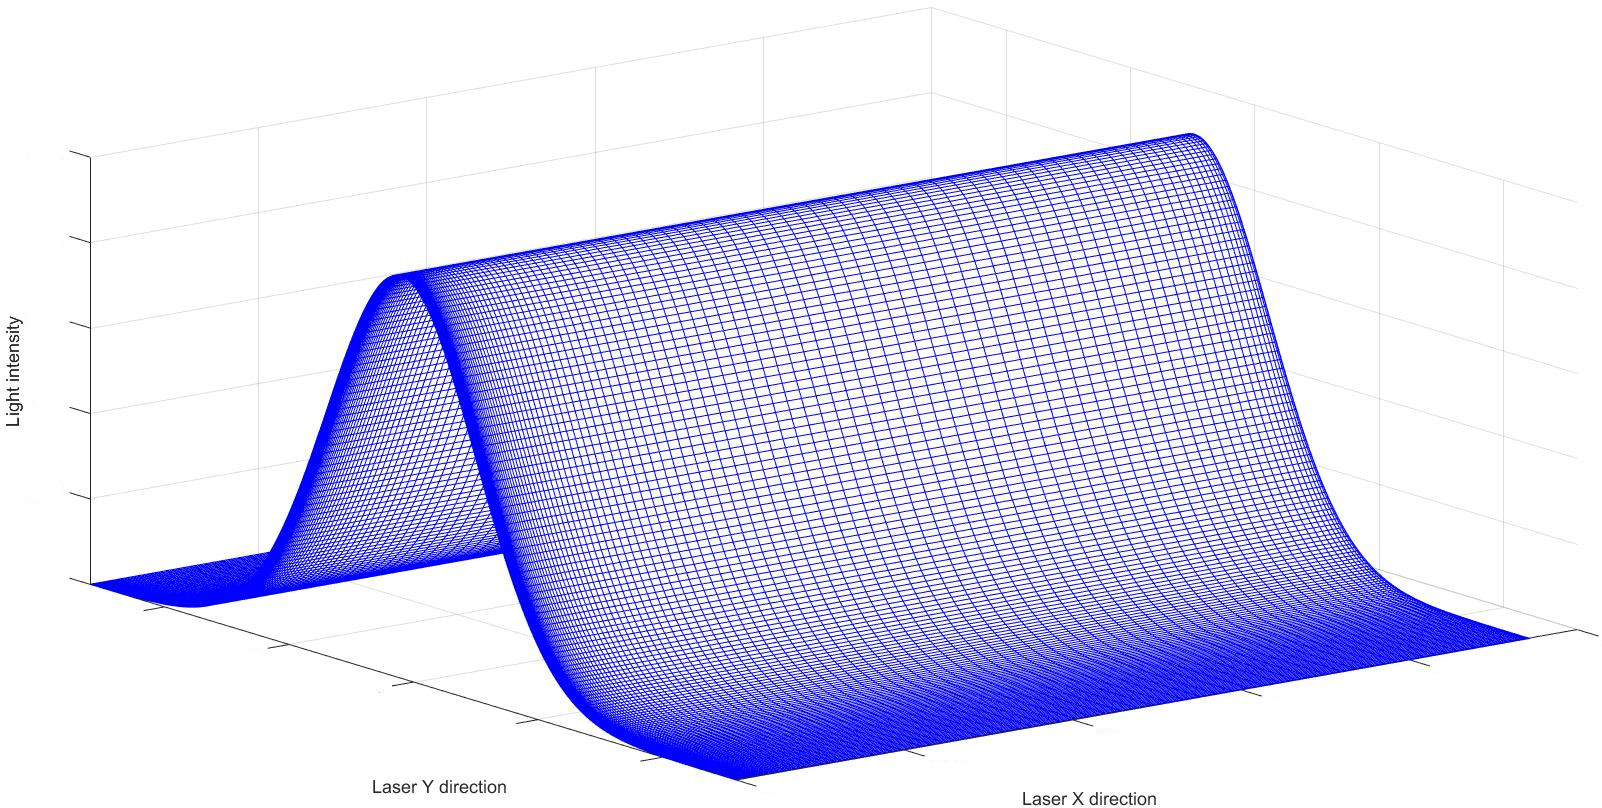
\includegraphics[width=0.8\textwidth]{./images/model/3Dgauss_grid.jpg}
    \caption{3D model of the laser line}
    \label{fig:mod-laser-line}
  \end{figure}
As we can see, we haven't any information about the position of the laser spot along the abscissa, so the only way to estimate the committed error is to use the distribution above. Thus, we modelled our error as follows:
  \begin{equation*}
    \sigma_{x_{c_i}} = \sqrt{\frac{\left(pixel \,\, size \right)^2}{12}}
  \end{equation*}
where the $pixel \,\, size$ is the ideal size of the pixel (along the $x$ axis if we assume it rectangular shaped). \\

A similar analysis can be made along the ordinate. However, even in conditions like the one shown in Figure \ref{fig:mod-laser-line}, along the ordinate we have always some informations about the shape of the laser line. This suggested us that it should be possible to consider all the mathematical models discussed in Subsection \ref{subsec:peak-detection}. In this way we should improve the detection of the laser spot peak, reducing the initial error. \\
In \cite{Naidu1991}, the authors present an interesting study on the precision of the approximations that we have considered above, nevertheless we are not convinced of the results they have achieved:
  \begin{itemize}
    \item First of all, we think that some of the proposed forms of $\hat{\delta}$ are incorrect. To validate our hypothesis, we evaluated from scratch each proposed filters. We reported our result in Table \ref{tab:local-mod}. As we can see, in particular for what concerns the approximation thought by Blaise and Rioux, the proposed model is too simplified. Short tests shown that the simplification made by \cite{Naidu1991} are too strong to be negligible, and from our point of view, they could be a source of errors. Furthermore, proposed results was estimated using a first-order approximation of the Gaussian, which further simplifies the problem. In short, we concluded that the problems are more complex than the paper shown.
    \item For each proposed model, the authors introduce a different constant, called $\alpha$, that allows to improve arbitrarily the filters performance. We noticed that they don't explain how they reached their results, and it seems that the value of $\alpha$ changes if we change the width of the laser spot: from a design point of view this is not acceptable.
    \item The proposed results were evaluated only in a specific condition (laser $\sigma \in \begin{bmatrix} 0.5 & 1 & 1.5 \end{bmatrix}$), which seems to be out of the actual working conditions.
  \end{itemize}
Hence, we decided to pass over suggested evaluations, and we looked for an alternative solution. \\
  \begin{table}[t!]
  \centering
  \begin{tabular}{|ccc|}

  \hline
  \textbf{Estimator}          & \textbf{Window} & \textbf{Local Estimator} \\
  \hline
  & & \\
  \textit{Gaussian}           & 3               &  $\delta$                \\ 
  & & \\ % \hline
  \textit{Linear}             & 3               & $\frac{\delta}{\sigma^2} \frac{e^{-\frac{1}{2\sigma^2}}}{1 - \left( 1 - \frac{\delta}{\sigma^2} \right) e^{-\frac{1}{2\sigma^2}}}$ \\ 
  & & \\ % \hline
  \textit{Parabolic}          & 3               & $\frac{\delta}{2\sigma^2} \frac{e^{-\frac{1}{2\sigma^2}}}{1-e^{-\frac{1}{2\sigma^2}}}$ \\ 
  & & \\ % \hline
  \textit{Center of Mass}     & 3               & $ \frac{2\delta}{\sigma^2} \frac{ e^{-\frac{1}{2\sigma^2}} }
                                                                         {  1+2e^{-\frac{1}{2\sigma^2}} }$ \\ 
  & & \\ % \hline
  \textit{Center of Mass}     & 5               & $ \frac{2\delta}{\sigma^2} \frac{ e^{-\frac{1}{2\sigma^2}} + 4e^{-\frac{4}{2\sigma^2}} }
                                                                         {1 + 2e^{-\frac{1}{2\sigma^2}} + 2e^{-\frac{4}{2\sigma^2}} }$ \\ 
  & & \\ % \hline
  \textit{Center of Mass}     & 7               & $\frac{2\delta}{\sigma^2} \frac{ e^{-\frac{1}{2\sigma^2}} + 4e^{-\frac{4}{2\sigma^2}} + 9e^{-\frac{9}{2\sigma^2}} }
                                                                        { 1 + 2e^{-\frac{1}{2\sigma^2}} + 2e^{-\frac{4}{2\sigma^2}} + 2e^{-\frac{9}{2\sigma^2}} }$ \\ 
  & & \\ % \hline
  \textit{Blais-Rioux}        & 4               &  $ -\frac{2\delta}{\sigma^2} \frac{ e^{-\frac{1}{2\sigma^2}} + 2e^{-\frac{1}{2\sigma^2}}}
  { -\frac{2\delta}{\sigma^2}e^{-\frac{1}{2\sigma^2}} - \frac{4\delta}{\sigma^2}e^{-\frac{4}{2\sigma^2}} 
    - f(\delta, \sigma)
  }$ \\
  \multicolumn{3}{|c|}{ $f(\delta, \sigma) =
      \left(1-\frac{\delta}{\sigma^2}\right)e^{-\frac{1}{2\sigma^2}}
      + 1
      - \left( 1+\frac{2\delta}{\sigma^2} \right)e^{-\frac{4}{2\sigma^2}}
      - \left( 1+\frac{3\delta}{\sigma^2} \right)e^{-\frac{9}{2\sigma^2}}
  $ } \\
  & & \\ 
  \hline
  \end{tabular}
  
  \caption{Table of local estimators $\hat{\delta}$, estimated for some of the proposed filters}
  \label{tab:local-mod}
\end{table}

In order to complete our model, we want to determine how much the peak approximation moves to its real position. As we can see in Table \ref{tab:local-mod}, we can write:
  \begin{equation*}
    \hat{\delta} = f(\sigma) \cdot \delta
  \end{equation*}
where $\delta$ is the real peak position inside the pixel, $\sigma$ is the standard deviation of the Gaussian and $f(\sigma)$ is a correction function. From this equation we can observe that the deviation $\epsilon$ of $\hat{\delta}$ from $\delta$ can be estimated as:
  \begin{equation*}
    \left| \epsilon \right| = \left| 1 - f(\sigma) \right| \cdot \left| \delta \right|
  \end{equation*}
If we consider the hypothesis that $\delta \in \left[ -\frac{1}{2}, \frac{1}{2}\right]$, given the pixel with the higher light intensity, and that the error is maximum when the peak is located between two pixels, we can conclude that the error committed by evaluating the peak position along the $y$ direction is given by:
  \begin{equation*}
    \sigma_{y_{c_i}} = \frac{1}{2} \cdot \left| 1 - f(\sigma) \right|
  \end{equation*}

In order to solve the problems introduced by the first-order approximation of the Gaussian, we thought to estimate as precise as possible the discrete Gaussian centered in $\delta = \frac{1}{2}$ and to use this signal as input of our implementations of the approximation filters. In this way we limited the sources of errors only to the approximation of the laser and not to the filter. \\

Another advantage of our approach is that it allows to consider saturation conditions. In real scenarios it might be that the laser is light-hearted out of focus; this is typical when we work at the limit of the depth of field of the laser. It is immediately understood that in these cases the approximation discussed above cannot work. To consider also these situations in our model, we modelled the saturated Gaussian signal as follows:
  \begin{equation*}
    \mathcal{N} = \left\{
      \begin{matrix}
        \frac{B}{A} & if \, |y| < \frac{A}{2} \\ 
        \frac{1}{\sqrt{2}\varsigma} e^{ - \frac{ (y - \delta )^2}{2\varsigma^2} } & otherwise \\
      \end{matrix}
    \right.
  \end{equation*}
where $y$ is the pixel coordinate; $\delta$ is the real sub-pixel position of the laser peak; $\varsigma$ is the Gaussian standard deviation; while $B$ and $A$ are respectively the saturation magnitude and aperture. \\
To completeness, we reported in Equations \ref{eq:sat-com5-err} and \ref{eq:sat-br4-err} a couple of examples of the effects of this new model. The interesting things are not the changes in approximations of $\hat{\delta}$ (that we expected), but the fact that what has been discussed so far continues to be valid: if we set $A = 0$, $\mathcal{N}$ is a general Gaussian distribution.
  \begin{equation}
    \hat{\delta}_{COM_5} \approx
    \frac{8\delta}{\sigma^2} \cdot \frac{
      e^{-\frac{4}{2\sigma^2}}
    }{
      \frac{3B}{A} + 2e^{-\frac{4}{2\sigma^2}}
    }
    \label{eq:sat-com5-err}
  \end{equation}
  \begin{equation}
    \hat{\delta}_{BR_4} \approx \frac{4\delta}{\sigma^2} \cdot \frac{
      e^{-\frac{4}{2\sigma^2}}
    }{
      \frac{2B}{A} -
      e^{-\frac{4}{2\sigma^2}} -
      e^{-\frac{9}{2\sigma^2}}
    }
    \label{eq:sat-br4-err}
  \end{equation}

\bigskip
Before concluding this section, we want to discuss about the Bessel approximation of the spot laser. Omitting the mathematical point of view, we noticed that the shape of this model is very similar to the one of the Gaussian. Accordingly with \cite{Naidu1991}, a good practise is to filter the images, in order to remove the noise of the camera, before applying the sub-pixel filters. Starting from these conditions, we hypothesized that if the minor crests are lower than the threshold of the filters, what we obtain after the filtering process is a rough approximation of a Gaussian signal. \\
The results of these tests are reported in Chapter \ref{ch:experimets}, however, for the moment we can only say that the hypothesis has been validated, hence no further analysis has been made on this model.
